\chapter{Capacity Test}
L'obiettivo del Capacity Test è quello di valutare le performance di un qualsiasi sistema quando è sottoposto a carichi di lavoro di diversa intensità, in modo da caratterizzare le sue prestazioni al limite (sotto condizioni di lavoro severe).
\\
Per realizzare queste valutazioni sono necessari gli \textbf{high-level parameters}, ovvero tutti quei parametri reperibili ed osservabili lato client. Essi possono riferirsi alla richiesta (quando è stata fatta, chi l'ha fatta ecc..) o alla risposta (tempi di risposta, errori).
\\
Essendo il sistema in questione un server, si è scelto di descrivere le sue performance attraverso:
\begin{enumerate}
	\item \textbf{Response Time}, intervallo di tempo che intercorre tra l'istante in cui il client inoltra la richiesta e quello in cui riceve la risposta.
	\item \textbf{Throughput}, richieste servite correttamente per unità di tempo.
\end{enumerate}
L'andamento atteso da parte di queste due metriche è il seguente:
\begin{figure}[H]
	\centering
	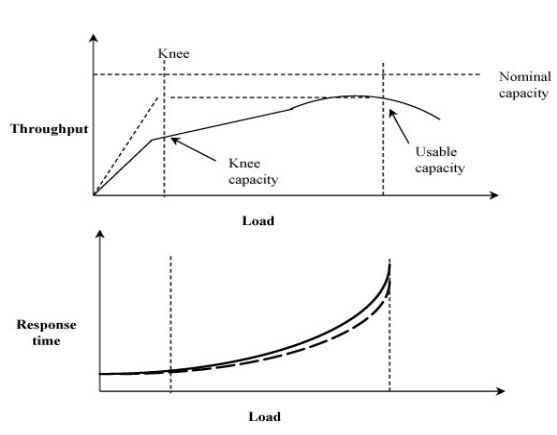
\includegraphics[width=0.8\textwidth]{img/hw2/Thr_resp.png}
	\caption{\textit{Grafici Throughput e Response time}}
\end{figure}
Di nostro interesse sono i valori di:
\begin{itemize}
	\item \textit{Knee Capacity}, punto prima del quale il throughput cresce linearmente all'aumentare del carico, ma il tempo di risposta non varia significativamente ed oltre il quale il guadagno in throughput è basso mentre il tempo di risposta aumenta con il carico.
	\item \textit{Usable Capacity}, massimo throughput raggiungibile portando il sistema al limite, senza eccedere un dato tempo di risposta.
\end{itemize}
Per ottenere agevolmente la Knee Capacity, viene introdotto un terzo parametro, la \textit{Potenza}. 
\\
\begin{equation}
	Power = \frac{Throughput}{Response Time}
\end{equation}
Tale punto coincide con il punto di massimo della potenza e rappresenta l'ottimo in corrispondenza del quale conviene operare per ottenere le prestazioni migliori.
\begin{figure}[H]
	\centering
	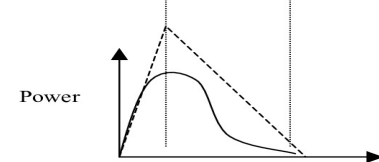
\includegraphics[width=0.5\textwidth]{img/hw2/Power.png}
	\caption{\textit{Grafico Potenza}}
\end{figure}


\section{Experimental Setup}
Il sistema oggetto di studio è un \textit{Web Server Apache} installato sulla macchina virtuale guest, che funge da server.
\\
Tramite la modalità \textit{Host-only Network Adapter}, configurabile nelle impostazioni della macchina virtuale, è stato possibile far comunicare la macchina guest con quella host, che lo ospita. Su quest'ultima è stata installata l'applicazione Java \textit{JMeter}, che ha permesso l'analisi delle prestazioni complessive del Server, sottoponendolo a diversi tipi di carico.
\\
\\
In questa analisi è stato scelto di valutare le prestazioni in media del server, considerando solo richieste di tipo random (tipo = dimensione pagina, nel nostro esempio). 
\subsection{Server Setup}
Descrizione configurazione VM - non la so.
\\
Per creare un scenario reale, sul Server sono state caricate 5 pagine in formato testuale, di diversa dimensione:
\begin{itemize}
	\item \textbf{Small}, 50K
	\item \textbf{Small-Medium}, 100K
	\item \textbf{Medium}, 300K
	\item \textbf{Medium-Large}, 500K
	\item \textbf{Large}, 1M
\end{itemize}
Questi sono i file oggetto delle richieste realizzate da ipotetici client.
\subsection{Clients - JMeter Setup}
Innanzitutto è stato settato, nel \textit{ThreadGroup}, il numero di thread che JMeter usa per realizzare i test. Questa quantità rappresenta il numero di utenti "virtuali" che visitano il nostro server. Nel nostro esperimento sono stati previsti \textbf{50 threads}, un valore in linea con i suoi scopi (visto che il sito fa un po'schifo non è che può avere tantissimi utenti). In più, prevedendo dei test di durata pari a \textit{5 min}, sono stati impostati:
\begin{itemize}
	\item il \textbf{ramp-up period} - numero di secondi entro il quale deve essere attivato l'ultimo thread - a \textit{300 s}. Ciò ci ha permesso di dilazionare l'attivazione degli utenti nei 5 minuti.
	\item il \textbf{thread lifetime} - durata massima di ogni thread - a \textit{300 s}.
	\item il \textbf{loop count} - numero di volte in cui un singolo thread viene attivato - a \textit{carico/50}.
\end{itemize}     
Al ThreadGroup sono stati aggiunti 5 \textit{HTTP Request Sampler}, uno per tipologia di richiesta da realizzare e nei quali sono stati specificati i path delle rispettive risorse sul server. Ad essi è stato integrato un \textit{Random Controller}, grazie al quale, quando un thread viene attivato, effettua solo una tra le cinque tipologie di richieste, selezionata in maniera randomica. Ancora una volta, aggiungendo variabilità alle nostre richieste, è stato possibile simulare una situazione realistica e, soprattutto, non predicibile.
\\
Attraverso il \textit{Constant Throughput Timer} è stato possibile impostare il carico da sottoporre al sistema, in termini di numero di richieste al minuto. Infine, il listener \textit{Simple Data Writer}, ci ha permesso di collezionare in un file, quei parametri di alto livello che sono d'interesse ai fini dell'esperimento.

\section{Esecuzione Capacity Test}
Inizialmente sono stati effettuati dei test il cui scopo era quello di far operare il Web Server "al limite". Ci si è resi conto che il massimo valore di carico entro il quale il sistema risponde adeguatamente (in quelle condizioni), è di circa \textit{6000 richieste al minuto}. 
\\
A partire da questo limite e ragionando sull'andamento di throughput e response time, si sono scelti i seguenti valori di carico da sottoporre al sistema:
\begin{equation}
	workloads = {100, 500, 800, 1000, 2000, 3000, 4000, 5000, 6000, 7000, 8000, 9000}
\end{equation}
Gli ultimi tre carichi (7000, 8000 e 9000 richieste al minuto) hanno permesso di evidenziare nei grafici il degradamento delle prestazioni del sistema.
\\
Per ogni valore di carico è stato calcolato il \textbf{Throughput}:
\begin{equation}
	Throughput = \frac{NumeroRichieste}{Timestamp(N) - Timestamp(1)} \frac{N}{s}
\end{equation}
Il \textit{timestamp} fa parte degli high-level parameters collezionati dal Simple Data Writer, e corrisponde all'istante di tempo (in millisecondi poi convertito in secondi) in cui il client ha inoltrato una data richiesta.
\\
Come \textbf{Response Time} è stato scelto il parametro \textit{Elapsed}, coincidente con il tempo che intercorre tra la sottomissione della richiesta da parte del client e la risposta del server. Dato che contiene anche il tempo di elaborazione della richiesta da parte del server, esso cresce all'aumentare della dimensione dei file richiesti, oltre che all'aumentare del carico.
\\
\\
Ogni misurazione (per ogni carico) è stata ripetuta \textbf{3 volte} in modo da tenere traccia dell'errore, e notando che i dati ottenuti non differivano di molto tra loro, come indice di posizione è stata scelta la loro media.
\\
\subsection{Risultati}
I file .csv sono stati caricati in uno script Matlab tramite cui sono stati automatizzati i procedimenti descritti sopra, i parametri sono stati plottati in funzione del carico considerato.
\\
\begin{figure}[H]
	\centering
	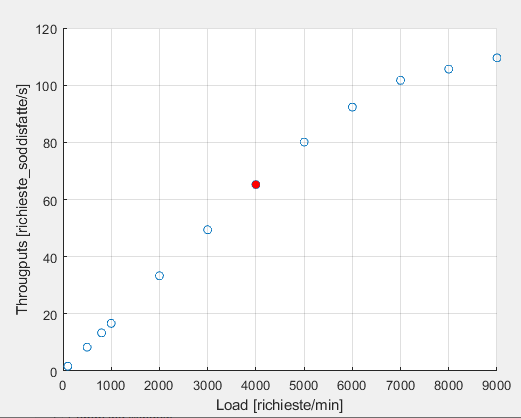
\includegraphics[width=0.8\textwidth]{img/hw2/Throughput.png}
	\caption{\textit{Grafico Throughput}}
\end{figure}

\begin{figure}[H]
	\centering
	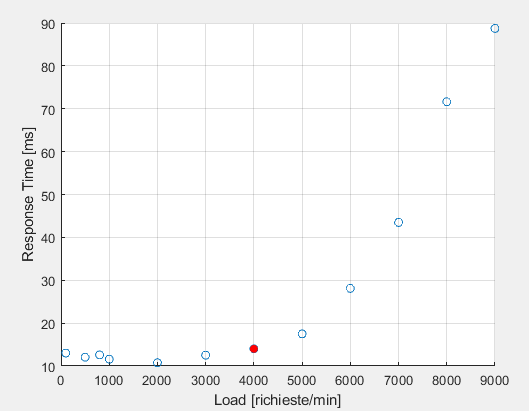
\includegraphics[width=0.8\textwidth]{img/hw2/ResponseTime.png}
	\caption{\textit{Grafico Response Time}}
\end{figure}

\begin{figure}[H]
	\centering
	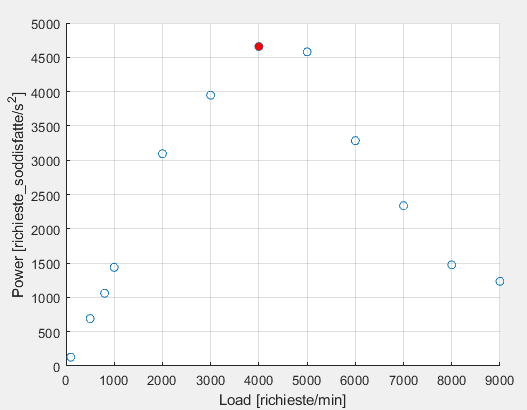
\includegraphics[width=0.8\textwidth]{img/hw2/Potenza.png}
	\caption{\textit{Grafico Potenza}}
\end{figure}
\newpage

Come si evince dal grafico della Potenza, il suo punto di massimo è associato ad un carico di 4000 richieste/min. 
\\
La \textit{Knee Capacity} (in rosso nel grafico dei Throughputs) è il valore throughput associato a questo carico. Ciò significa che se il nostro server opera in condizioni ottimali riesce a soddisfare circa 65,2112 richieste al secondo, ovvero 3836 richieste al minuto mediamente.
\\

Per quanto riguarda il calcolo della \textit{Usable Capacity}, possiamo relazionarla al tempo di risposta del server quando è sottoposto ad un carico di 6000 richieste/min (il carico limite). Questo response time è pari a 28,11 ms e coincide con quel tempo oltre il quale il sistema inizia a non rispondere più adeguatamente. Pertanto, la Usable Capacity può essere espressa come il valore di throughput associato al carico limite, ovvero 92,3314 richieste al secondo (5431 richieste al minuto circa).
\\
Ovviamente il valore di carico a cui conviene far lavorare il nostro Web Server non è quello massimo che riesce a soddisfare (Usable Capacity). Difatti non sarebbe efficiente per due motivi:
\begin{enumerate}
	\item i tempi di risposta associato a tale carico sono elevati.
	\item essendo il carico limite, basta poco per ricadere nella zona di minima efficienza. (scrivere meglio)
\end{enumerate}
